\section{Experiments}
\label{sec:experiments}

\subsection{Single-Frame MOT Benchmark}

\paragraph{Setup.} Random similarity matrices 
$p \in [0,1]^{T \times D}$ with $T = D \in \{10, 20, 30, 50\}$.

\begin{table}[t]
    \centering
    \caption{Single-frame MOT: solution quality and computation time.}
    \label{tab:single-frame}
    \begin{threeparttable}
    \begin{tabular}{l S[table-format=-2.2] S[table-format=-2.2] 
                    S[table-format=-2.2] }
        \toprule
        \multirow{2}{*}{Size $T=D$} & 
        \multicolumn{3}{c}{Assignment cost} \\
        \cmidrule(lr){2-4}
        & {Hungarian} & {Greedy} & {\ZSP} \\
        \midrule
        10 & -8.60 & -7.95 & -8.59 \\
        20 & -18.46 & -17.52 & -18.46 \\
        30 & -28.51 & -27.07 & -28.50 \\
        50 & -48.39 & -46.77 & -48.37 \\
        \bottomrule
    \end{tabular}
    \end{threeparttable}
\end{table}

\begin{table}[t]
    \centering
    \caption{Single-frame MOT: computation time (ms).}
    \label{tab:single-frame-time}
    \begin{tabular}{l S[table-format=0.2] S[table-format=4.2] 
                    S[table-format=5.0] }
        \toprule
        Size $T=D$ & {Hungarian} & {\ZSP} & {Ratio} \\
        \midrule
        10 & 0.01 & 34.56 & 3456 \\
        20 & 0.01 & 65.14 & 6514 \\
        30 & 0.03 & 222.27 & 7409 \\
        50 & 0.07 & 1498.87 & 21412 \\
        \bottomrule
    \end{tabular}
\end{table}

\paragraph{Result.} \ZSP achieves $99.96\%$ of Hungarian's solution 
quality but is $3456$--$21412\times$ slower 
(\cref{tab:single-frame,tab:single-frame-time}). 
See \cref{fig:single-frame} for visual comparison.

\begin{figure}[t]
    \centering
    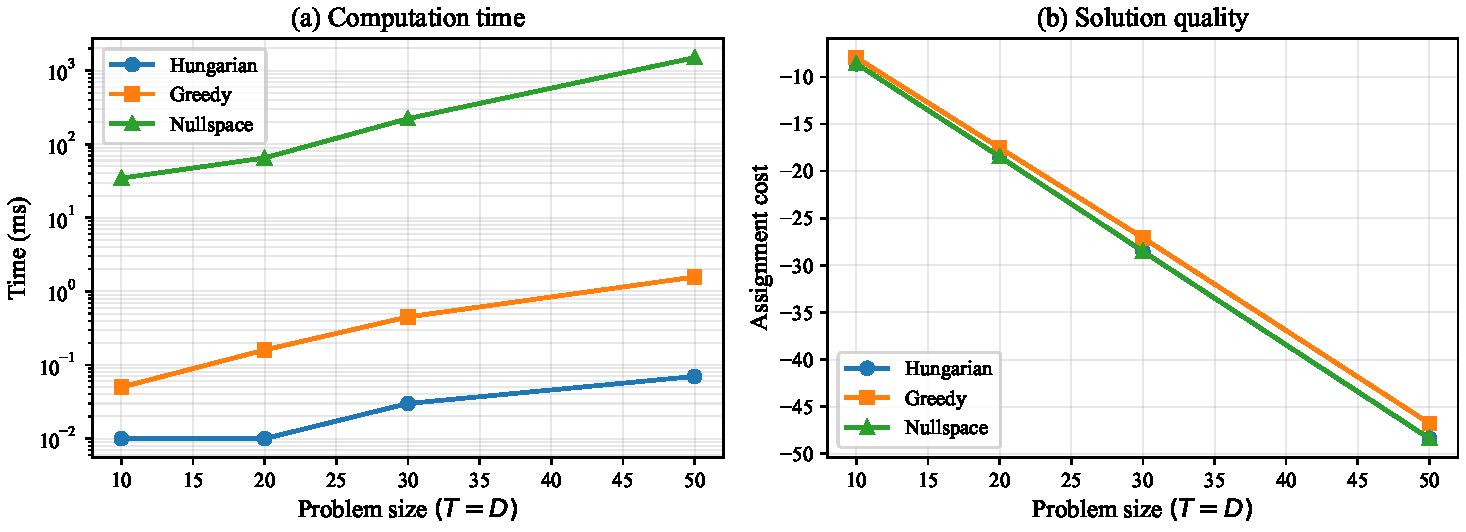
\includegraphics[width=\linewidth]{figures/fig2_single_frame.pdf}
    \caption{Single-frame MOT: (a) computation time on log scale; 
    (b) solution quality. Hungarian is both faster and (marginally) 
    more accurate than \ZSP.}
    \label{fig:single-frame}
\end{figure}

\subsection{Multi-Frame MOT Benchmark}

\paragraph{Setup.} Synthetic data with $K$ frames, $T$ tracks, $D$ 
detections, incorporating miss detections ($25\%$), false positives 
($15\%$), and occlusion ($20\%$). We run 30 seeds per configuration.

\begin{table}[t]
    \centering
    \caption{Multi-frame MOT: statistical comparison across 30 seeds.}
    \label{tab:multiframe}
    \begin{tabular}{l S[table-format=1.3] S[table-format=1.3] 
                    S[table-format=+1.3] }
        \toprule
        Metric & {Hungarian} & {\ZSP} & {Difference} \\
        \midrule
        Mean accuracy & 0.909 & 0.842 & -0.067 \\
        Std. deviation & 0.122 & 0.129 & --- \\
        $t$-statistic & \multicolumn{2}{c}{$-4.580$} & \\
        $p$-value & \multicolumn{2}{c}{$0.0001$} & \\
        Win rate & \multicolumn{2}{c}{$0\%$} & \\
        \bottomrule
    \end{tabular}
\end{table}

\paragraph{Result.} \ZSP is \emph{statistically significantly worse} 
than Hungarian ($-6.7\%$, $p=0.0001$), with zero wins across 
30 seeds (\cref{tab:multiframe,fig:multiframe}).

\begin{figure}[t]
    \centering
    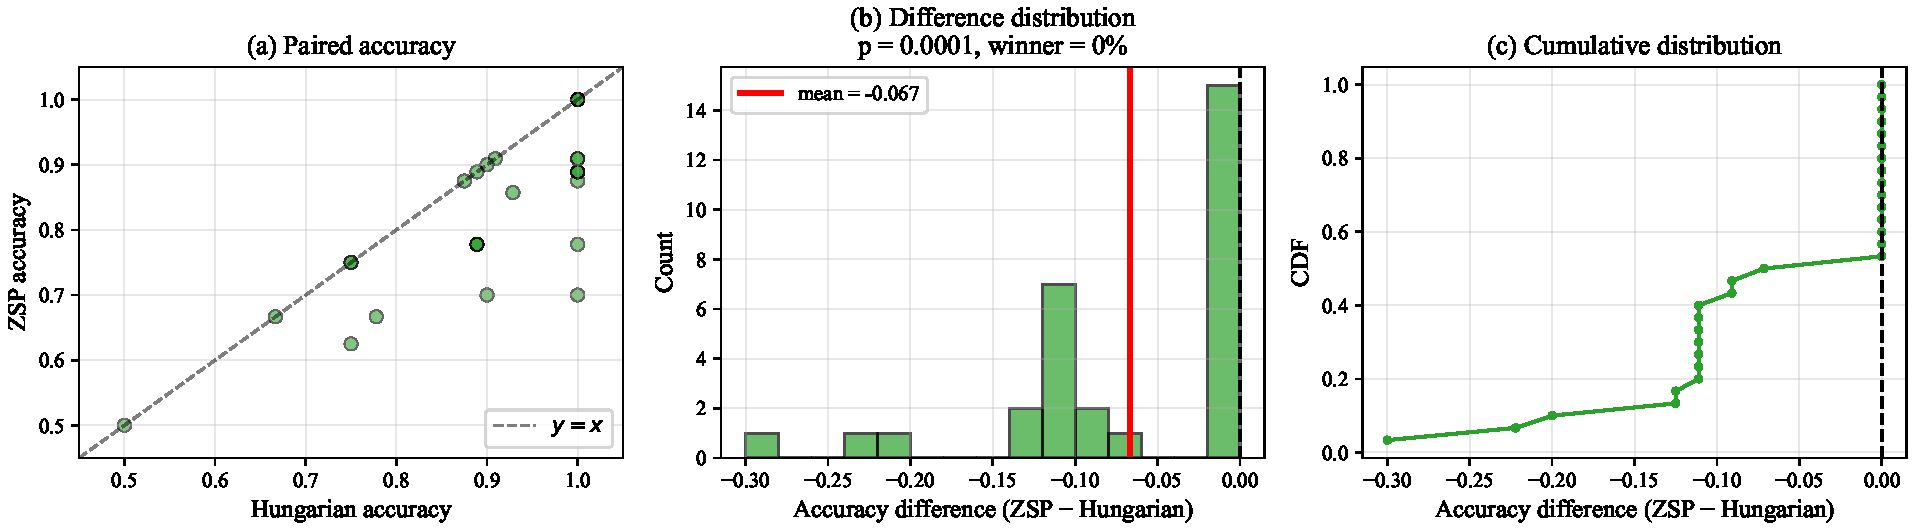
\includegraphics[width=\linewidth]{figures/fig3_multiframe.pdf}
    \caption{Multi-frame MOT: (a) paired accuracy scatter; 
    (b) difference distribution; (c) CDF. \ZSP is systematically 
    worse than Hungarian.}
    \label{fig:multiframe}
\end{figure}

\subsection{Cooperative Perception Benchmark}

\paragraph{Setup.} $M$ vehicles, each with $T$ tracks and $D$ 
detections, sharing boundary data.

\begin{table}[t]
    \centering
    \caption{Cooperative perception: accuracy, time, communication.}
    \label{tab:cooperative}
    \begin{tabular}{l l S[table-format=1.3] S[table-format=3.2] 
                    S[table-format=4.0]}
        \toprule
        Config & Method & {Accuracy} & {Time (ms)} & {Comm (B)} \\
        \midrule
        \multirow{3}{*}{$M{=}2,T{=}6,D{=}8$} 
            & Central.\ Hung. & 1.000 & 21.71 & --- \\
            & Distrib.\ Hung. & 1.000 & 0.03 & 0 \\
            & Distrib.\ \ZSP & 1.000 & 15.99 & 480 \\
        \midrule
        \multirow{3}{*}{$M{=}3,T{=}8,D{=}10$} 
            & Central.\ Hung. & 1.000 & 0.82 & --- \\
            & Distrib.\ Hung. & 1.000 & 0.04 & 0 \\
            & Distrib.\ \ZSP & 1.000 & 26.22 & 960 \\
        \midrule
        \multirow{3}{*}{$M{=}4,T{=}10,D{=}12$} 
            & Central.\ Hung. & 1.000 & 1.56 & --- \\
            & Distrib.\ Hung. & 1.000 & 0.05 & 0 \\
            & Distrib.\ \ZSP & 1.000 & 71.23 & 1600 \\
        \bottomrule
    \end{tabular}
\end{table}

\paragraph{Result.} All methods achieve $100\%$ accuracy, but 
distributed Hungarian is fastest and requires zero communication 
(\cref{tab:cooperative,fig:cooperative}).

\begin{figure}[t]
    \centering
    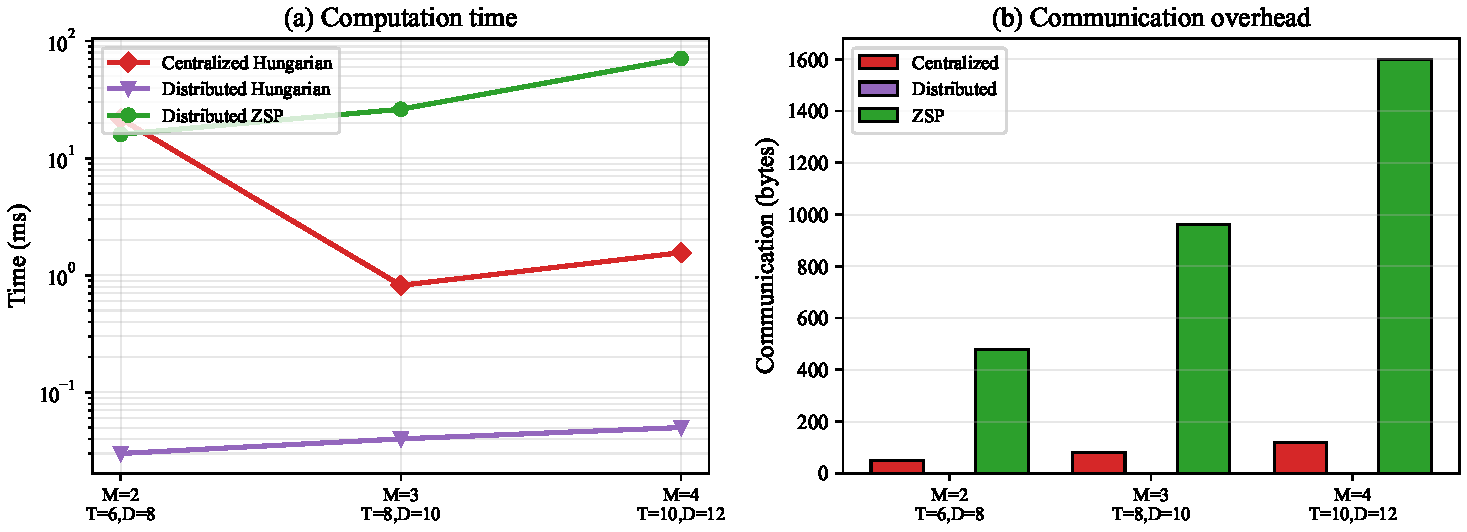
\includegraphics[width=\linewidth]{figures/fig4_cooperative.pdf}
    \caption{Cooperative perception: (a) computation time on log 
    scale; (b) communication overhead. Distributed Hungarian 
    dominates on both metrics.}
    \label{fig:cooperative}
\end{figure}

\subsection{Noise Resilience}

\begin{figure}[t]
    \centering
    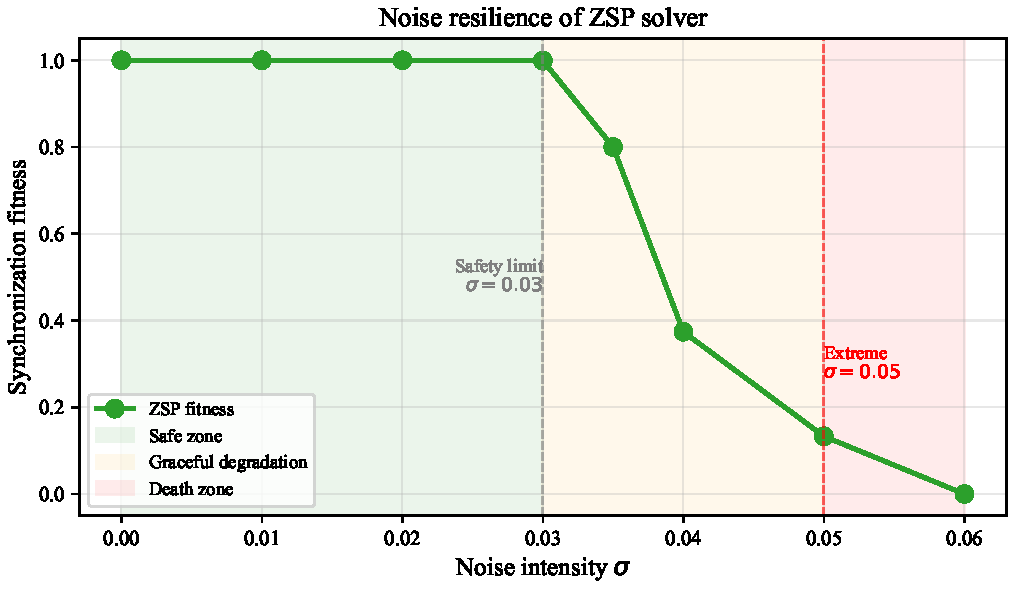
\includegraphics[width=0.75\linewidth]{figures/fig5_noise.pdf}
    \caption{Noise resilience of \ZSP solver: synchronization 
    fitness vs.\ noise intensity $\sigma$. Safe operation up to 
    $\sigma = 0.03$; graceful degradation zone from $0.03$ to $0.05$.}
    \label{fig:noise}
\end{figure}

\subsection{Digital-Twin Verification}

\begin{figure}[t]
    \centering
    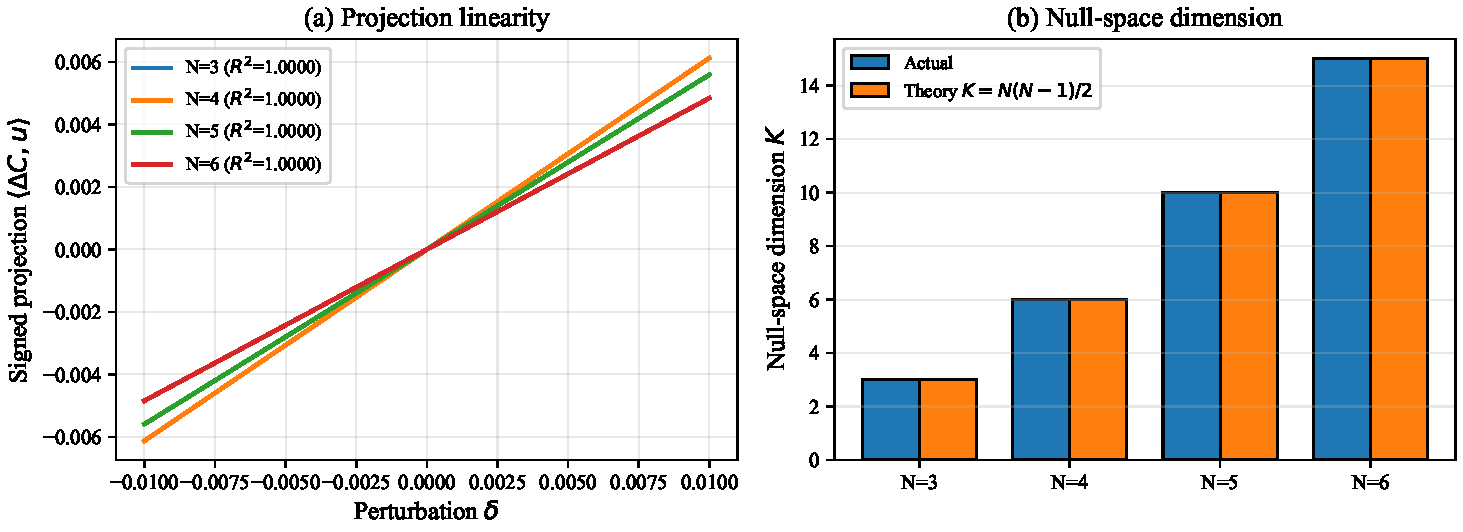
\includegraphics[width=\linewidth]{figures/fig1_digital_twin.pdf}
    \caption{Digital-twin verification of \abnqss v3.0: 
    (a) projection linearity $R^2 = 1.000000$; 
    (b) null-space dimension $K = N(N-1)/2$. Both match theory exactly.}
    \label{fig:digital-twin}
\end{figure}